%% Bookheader, Nov 8, 2020; July 18, 2022

\documentclass[11pt]{../Support/ourbook}
%% or for landscape, comment out line above and use this one:
%%\documentclass[landscape,11pt]{ourbook}

%% This will keep space from stretching around display math:

\makeatletter
\renewcommand\normalsize{%
   \@setfontsize\normalsize\@xipt{13.6}%
   \abovedisplayskip 11\p@  \@minus6\p@
   \abovedisplayshortskip \z@ 
   \belowdisplayshortskip 6.5\p@ \@minus3\p@
   \belowdisplayskip \abovedisplayskip
   \let\@listi\@listI}
\makeatother
\normalsize


\begin{document}

\tableofcontents
\graphicspath{{../../Chapters/limits/en_US}}
	\chapter{Limits}

The asymptotic behavior we see in rational functions suggests that we need to expand our vocabulary of function characteristics. We examined vertical asymptotes and end behavior through graphs and tables and discussed them in English. The language of limits enables us to discuss these attributes with greater efficiency. 

Let us revisit an example from the previous chapter. This function has a hole at $ x = 1 $, a vertical asymptote at $ x = 3 $, and a horizontal asymptote of $ y = 1 $.

$$ f(x) = \frac{x^2 - 3x + 2}{x^2 - 4x + 3} = \frac{(x-1)(x-2)}{(x-1)(x-3)} $$

\begin{figure}[htbp]
  \centering
  \begin{tikzpicture}
    \begin{axis}[
	  xmin=-5, xmax=5,
	  ymin=-5, ymax=5,
      axis lines = middle,
      xlabel = \(x\),
      ylabel = \(f(x)\),
      restrict y to domain = -10:10,
      samples = 100,
    ]
    \addplot [blue, smooth] {(x - 2)/(x - 3)};
    \draw[dashed] (axis cs: 3,-5) -- (axis cs: 3,5);
    \draw[dashed] (axis cs: -5,1) -- (axis cs: 5,1);
    \end{axis}
  \end{tikzpicture}
  \caption{Graph of \( f(x) = \frac{x^2 - 3x + 2}{x^2 - 4x + 3} \) with asymptotes}
\end{figure}

First, consider the vertical asymptote. We see that the graph goes down as it hugs the left side of the vertical asymptote, and goes up as it hugs the right side. We can describe these behaviors as the left- and right-hand limits, respectively. We say that the left-hand limit of $ f $ at $ x = 3 $ is negative infinity. Another way of communicating this is to say that as $ x $ approaches $ 3 $ from the left, the function approaches negative infinity. Symbolically, we summarize this as $ \lim_{x \rightarrow 3^-} f(x) = -\infty $.

Similarly, the right-hand limit of $ f $ at $ x = 3 $ is positive infinity. In other words, as $ x $ approaches $ 3 $ from the right, the function approaches positive infinity. Symbolically, we write $ \lim_{x \rightarrow 3^+} f(x) = \infty $.

The limit of a function at a particular $ x $-value is the $ y $-value that the function approaches as it approaches the given $ x $-value. In the previous example, we could only specify the left- and right-hand limits, because they were different. In cases where the left- and right-hand limits are equal, we can say that the function has a limit there. The hole in our function $ f $ is one such value. We see that as we approach the hole from both the left and right, the function takes on values near $\frac{1}{2}$. This is more apparent numerically:


\begin{center}
\begin{tabular}{ |c|c|c|c|c|c|c|c| } 
 \hline
 x & 0.9 & 0.99 & 0.999 & 1 & 1.001 & 1.01 & 1.1 \\ 
 \hline
 f(x) & 0.5238 & 0.5025 & 0.5003 & undefined & 0.4998 & 0.4975 & 0.4737 \\ 
 \hline
\end{tabular}
\end{center}

The left-hand and right-hand limits of $ f $ at $ 1 $ are both $\frac{1}{2}$. Since they are equal, we can also say that the limit of $ f $ at $ 1 $ is $\frac{1}{2}$. This allows us to efficiently discuss the behavior of $ f $ at $ 1 $, even though the function is not defined there since substituting $ 1 $ into the function gives division by zero.

$$ \lim_{x \rightarrow 1^-} f(x) = \lim_{x \rightarrow 1^+} f(x) = \lim_{x \rightarrow 1} f(x) = \frac{1}{2} $$

We can also talk about limits at $x$-values where nothing weird is happening, that is, no hole or vertical asymptote. For example, as $x$ approaches $4$ from the left and right, $y$ approaches $2$.

\begin{center}
\begin{tabular}{ |c|c|c|c|c|c|c|c| } 
 \hline
 x & 3.9 & 3.99 & 3.999 & 4 & 4.001 & 4.01 & 4.1 \\ 
 \hline
 f(x) & 2.1111 & 2.0101 & 2.0010 & 2 & 1.9990 & 1.9901 & 1.9091 \\ 
 \hline
\end{tabular}
\end{center}

In this case, since nothing weird is happening, the limit is equal to the function value. This is an example of continuity, which we will discuss in more detail in the next chapter. By contrast, at the vertical asymptote $ x = 1 $, since the left- and right-hand limits are not equal, we say the function does not have a limit, or the limit does not exist.

Finally, let us consider the horizontal asymptote of $f$. The graph hugs the line $y = 1$ as $x$ goes far to the left and far to the right. We say that as $x$ approaches negative infinity, $f$ approaches $1$, and likewise, that as $x$ approaches positive infinity, $f$ approaches $1$. We write these symbolically as $\lim_{x \rightarrow -\infty} f(x) = 1$ and $\lim_{x \rightarrow \infty} f(x) = 1$. 

\begin{Exercise}[title=Limits Practice 1, label=limits1]
  Determine the left- and right-hand limits of the function as $x$ approaches the given values. At $x$-values where the limit exists, determine it.
  \Question{$p(x) = \frac{x + 3}{x^2 + 9x + 18}, x = -6, -5, -3, \infty$}
  \vspace{40mm}
\end{Exercise}
\begin{Answer}[ref=limits1] 
	$$ \lim_{x \rightarrow -6^-} p(x) = -\infty, \lim_{x \rightarrow -6^+} p(x) = \infty $$
	$$ \lim_{x \rightarrow -5^-} p(x) = \lim_{x \rightarrow -5^+} p(x) = \lim_{x \rightarrow -5} p(x) = 1 $$
	$$ \lim_{x \rightarrow -3^-} p(x) = \lim_{x \rightarrow -3^+} p(x) = \lim_{x \rightarrow -3} p(x) = \frac{1}{3} $$
	$$ \lim_{x \rightarrow \infty} p(x) = 0 \text{ called simply a limit, although it is a left-hand limit} $$
\end{Answer}

We have seen two weird behaviors of rational functions at certain $x$-values: holes and vertical asymptotes. Now we will examine another type of weird behavior: jumps. This is a characteristic of some piecewise defined functions. In piecewise defined functions, the domain is divided into two or more pieces, and a different expression is used to give the y-value depending on which piece contains the $x$-value. One common piecewise defined function is the floor function, sometimes denoted $\lfloor x \rfloor$. The standard floor function rounds any real number down to the nearest integer. So, for a price quoted in dollars and cents, the floor would be just the number of dollars.

\begin{figure}[htbp]
  \centering
	\begin{tikzpicture}
	\begin{axis}[
	    xmin=-5, xmax=5,
	    ymin=-5, ymax=5,
	    axis lines=middle,
	    xlabel={$x$},
	    ylabel={$y$},
	]
	\addplot[domain=-5:5, samples=500, blue] {floor(x)};
	\end{axis}
	\end{tikzpicture}
  \caption{Graph of \( y = \lfloor x \rfloor \)}
\end{figure}	

When $x$ is exactly $1$, the function value is $1$: the number of dollars in a price of \$1.00. When $x$ is any number greater than $1$ but less than $2$, the function value is still $1$. Also, $ \lfloor 1.01 \rfloor, \lfloor 1.5 \rfloor, \text{and} \lfloor 1.99999 \rfloor$ are all $1$. As we continue to look to the right, once $x$ equals exactly $2$, $h$ jumps up to the value $2$. So, $ \lim_{x \rightarrow 2^-} \lfloor x \rfloor = 1 $, while $ \lim_{x \rightarrow 2^+} \lfloor x \rfloor = 2 $.

Besides rational and piecewise defined functions, there are other functions with interesting limits. Consider the standard exponential function, $y = e^x$.

\begin{figure}[htbp]
  \centering
	\begin{tikzpicture}
	\begin{axis}[
	    xmin=-5, xmax=5,
	    ymin=-0, ymax=10,
	    axis lines=middle,
	    xlabel={$x$},
	    ylabel={$y$},
	]
	\addplot[domain=-5:5, samples=500, blue] {exp(x)};
	\end{axis}
	\end{tikzpicture}
  \caption{Graph of \( y = e^x \)}
\end{figure}	

As $x$ increases, $y$ increases without bound; that is, $\lim_{x \rightarrow \infty} e^x = \infty$. However, looking far to the left, we see that $y$ hugs the $x$-axis. This is because raising $e$ to a large negative exponent is the same as $1$ divided by $e$ raised to a large positive exponent; that is, $1$ divided by a very large number, which yields a very small positive number. In limit notation, $\lim_{x \rightarrow -\infty} e^x = 0$. This example illustrates that horizontal asymptotes need not model end behavior in both directions. Note that this reasoning holds for $y = b^x$ for any $b > 1$, so all such functions have the same horizontal asymptote, $y = 0$.

We know that the natural logarithm function, $y = \text{ln } x$, is the inverse of $y = e^x$. Since inverse functions swap the role of $x$ and $y$, it stands to reason that a horizontal asymptote in one function corresponds with a vertical asymptote in the other function, and that is indeed the case.

\begin{figure}[htbp]
  \centering
	\begin{tikzpicture}
	\begin{axis}[
	    xmin=0, xmax=10,
	    ymin=-5, ymax=5,
	    axis lines=middle,
	    xlabel={$x$},
	    ylabel={$y$},
	]
	\addplot[domain=0.001:10, samples=500, blue] {ln(x)};
	\end{axis}
	\end{tikzpicture}
  \caption{Graph of \( y = \text{ln } x \)}
\end{figure}	

An untransformed logarithm function is defined only for positive inputs. That is because it is not possible to find an exponent of a positive number which will yield a negative or zero result. What type of exponent on a positive number yields a number near zero? That would be a large-magnitude negative number. So, on the logarithm graph, large negative $y$-values correspond with $x$-values only slightly greater than zero. So, $\text{ln } x$ (and $\text{log}_2 x$, and indeed $\text{log}_b x$ for any $b > 1$) approaches negative infinity as $x$ approaches $0$ from the right. There is no left-hand limit at $0$, however. In limit notation, $\lim_{x \rightarrow 0^+} \text{ln } x = -\infty$.

\begin{Exercise}[title=Limits Practice 2, label=limits2]
  State the asymptotes of the following transformed exponential and logarithmic functions. Give the limit statement which describes the behavior of the function along the asymptote.
  \Question{$y = 3^x + 1, y = \text{log}_2 (x-4), y = 2^{1-x}, y = \text{log}_{10} (-2x)$}
  \vspace{40mm}
\end{Exercise}
\begin{Answer}[ref=limits2] 
	$$ \lim_{x \rightarrow -\infty} 3^x + 1 = 1; \lim_{x \rightarrow 4^+} \text{log}_2 (x-4) = -\infty; \lim_{x \rightarrow \infty} 2^{1-x} = 0; \lim_{x \rightarrow 0^-} \text{log}_{10} (-2x) = -\infty $$
\end{Answer}

We conclude this chapter by considering two functions which each have two horizontal asymptotes. These two seemingly obscure functions are quite important in data science.

\begin{figure}[htbp]
  \centering
  \begin{tikzpicture}
    \begin{axis}[
        xmin=-10, xmax=10,
        ymin=-2, ymax=2,
        axis lines=middle,
        xlabel={$x$},
        ylabel={$y$},
        xtick={-10,-5,...,10},
        ytick={-2,-1,...,2},
    ]
    \addplot[domain=-10:10, samples=200, blue] {rad(atan(x))};
    \draw[dashed] (axis cs:-10,1.5708) -- (axis cs:10,1.5708);
    \draw[dashed] (axis cs:-10,-1.5708) -- (axis cs:10,-1.5708);
    \end{axis}
  \end{tikzpicture}
  \caption{Graph of \(y = \arctan x\)}
\end{figure}

We know that the arctangent, or inverse tangent, function is the inverse of the piece of the tangent function which passes through the origin. The vertical asymptotes bounding this piece become horizontal asymptotes when the function is inverted.

Here are the equation and graph of the logistic function:

\begin{figure}[htbp]
  \centering
  \begin{tikzpicture}
    \begin{axis}[
        xmin=-10, xmax=10,
        ymin=0, ymax=1,
        axis lines=middle,
        xlabel={$x$},
        ylabel={$y$},
        xtick={-10,-5,...,10},
        ytick={0,0.5,1},
    ]
    \addplot[domain=-10:10, samples=200, blue] {1/(1+exp(-x))};
    \draw[dashed] (axis cs:-10,1) -- (axis cs:10,1);
    \draw[dashed] (axis cs:-10,0) -- (axis cs:10,0);
    \end{axis}
  \end{tikzpicture}
  \caption{Graph of the logistic function, $ y = \frac{1}{1 + e^{-x}} $}
\end{figure}

%\begin{figure}[htbp]
%  \centering
%  \begin{tikzpicture}
%    \begin{axis}[
%      axis lines = middle,
%      xlabel = \(x\),
%      ylabel = \( \frac{1}{1 + e^{-x}} \),
%      restrict y to domain = -5:5,
%      samples = 100,
%      xmin = -5, xmax = 5, ymin = 0, ymax = 1.1,
%    ]
%    \addplot [brown, smooth] {1/(1+exp(-x))};
%    \end{axis}
%  \end{tikzpicture}
%  \caption{Graph of the logistic function, $ y = \frac{1}{1 + e^{-x}} $ }
%\end{figure}

For large magnitude negative values of $x$, the exponential term in the denominator becomes a very large positive value. The fraction thus becomes a positive number very close to zero. For large magnitude positive values of $x$, that exponential term becomes a very small positive number. Adding it to $1$ yields a denominator just barely greater than $1$. Dividing $1$ by this number thus yields a function value just barely less than $1$. So, the logistic function yields values between $0$ and $1$, though never equaling either of these values exactly. It is precisely this characteristic which makes the logistic function so useful.

\begin{Exercise}[title=Limits Practice 3, label=limits3]
Using limit notation, state the limits as x approaches negative and positive infinity for the inverse tangent and logistic functions.
  \vspace{40mm}
\end{Exercise}
\begin{Answer}[ref=limits3] 
	$ \lim_{x \rightarrow -\infty} \text{tan}^{-1}x = -\frac{\pi}{2}, \lim_{x \rightarrow \infty} \text{tan}^{-1}x = \frac{\pi}{2}; \lim_{x \rightarrow -\infty} \frac{1}{1 + e^{-x}} = 0, \lim_{x \rightarrow \infty} \frac{1}{1 + e^{-x}} = 1 $
\end{Answer}

As seen above, the limit of a function from the left may be different from the limit of the function from the right. Additionally, the actual \textit{value} of the function may be different from the limit. Consider the piecewise function h(x):

$h(x) = \begin{cases}
    -x^2+3, \text{ if } x < 0\\
    2, x=0\\
    -x+3, \text{ if } x > 0
\end{cases}$

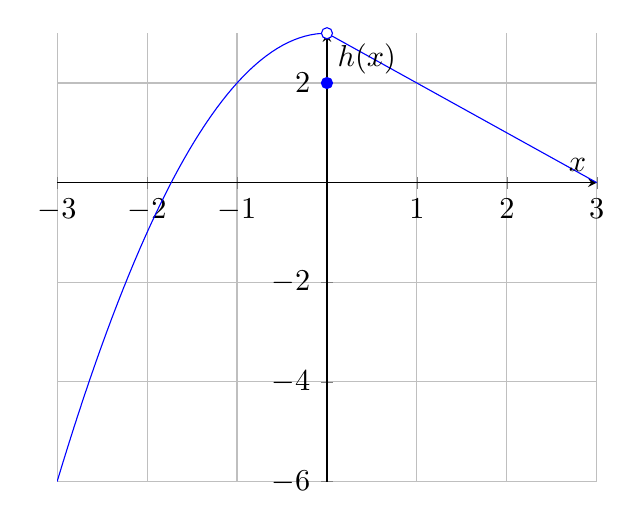
\begin{tikzpicture}
    \begin{axis}
        [grid, axis lines = center, xlabel = \(x\), ylabel=\(h(x)\)]
    \addplot[
    domain=-3:0,
    samples=50,
    color=blue,
    ]
    {-x^2+3};
    \addplot[mark=*,fill=white,draw=blue] coordinates{(0,3)};
    \addplot[mark=*,fill=blue,draw=blue] coordinates{(0,2)};
    \addplot[
    domain=0:3,
    samples=50,
    color=blue,
    ]
    {-x+3};
    \end{axis}
\end{tikzpicture}

From examining the graph, we see that $$\lim_{x\to0_-}h(x) = \lim_{x\to0_+}h(x) = 3$$
However, $h(0) = 2 \neq 3$. So, does this limit exist? It does! The limit of a function describes the \textit{behavior} of the function around a particular value, not the value of the function itself. In order for a limit to exist, the limits from the left and right must be equal to each other, but not necessarily the actual value of the function. 

Left and right limits practice: determine the limit from the left and the right for each function at the given value(s). State the limit at that value, if it exists. 
\begin{enumerate}
    \item $h(x), x=-1, 0, 1$
    \item $f(x), x=-1, 0, 2$
    \item $g(x), x=-2, 0, 1, 2$
\end{enumerate}

Solutions:
\begin{enumerate}
    \item $\lim_{x\to-1_-}h(x) = 2$ and $\lim_{x\to-1_+}h(x)=2$, therefore the limit exists and $\lim_{x\to-1}h(x)=2$

    $\lim_{x\to0_-}h(x) = 3$ and $\lim_{x\to0_+}h(x)=3$, therefore the limit exists and $\lim_{x\to0}h(x)=3$

    $\lim_{x\to1_-}h(x) = 2$ and $\lim_{x\to1_+}h(x)=2$, therefore the limit exists and $\lim_{x\to1}h(x)=2$
    \item $\lim_{x\to-1_-}f(x)=2$ and $\lim_{x\to-1_+}f(x)=2$, therefore the limit exists and $\lim_{x\to-1}f(x) = 2$.

    $\lim_{x\to0_-}f(x) = 3$ and $\lim_{x\to0_+}f(x) = 0$, and because $\lim_{x\to0_-}f(x) \neq \lim_{x\to0_+}f(x)$, the limit does not exist.

    $\lim_{x\to2_-}f(x) = -2$ and $\lim_{x\to2_+}f(x) = -2$, therefore the limit exists and $\lim_{x\to2}f(x) = -2$.

    \item $\lim_{x\to-2_-}g(x) = -1$ and $\lim_{x\to-2_+}g(x) = -1$, therefore the limit exists and $\lim_{x\to-2}g(x) = -1$.

    $\lim_{x\to0_-}g(x)=1$ and $\lim_{x\to0_+}g(x) = 1$, therefore the limit exists and $\lim_{x\to0}g(x) = 1$

    $\lim_{x\to1_-}g(x) = 2$ and $\lim_{x\to0_+}g(x) = 1$, and because $\lim_{x\to1_-}g(x) = 2 \neq \lim_{x\to0_+}g(x)$, the limit does not exist.

    $\lim_{x\to2_-}g(x) = 0$ and $\lim_{x\to2_+}g(x) = 0$, therefore the limit exists and $\lim_{x\to2}g(x) = 0$
\end{enumerate}

A quick note about continuity:

In order to be able to talk more about limits and know when we can apply certain rules and theorems, we first must discuss continuity. A function is continuous if there are no ``jumps'' or ``gaps'' in the graph of the function. For example, the function $f(x) = x^2$ is continuous for all real values of x. On the other hand, the function $g(x) = tan(x)$ has many discontinuities, including at $x=\frac{\pi}{2}$. Let's examine the graph of each of these functions:

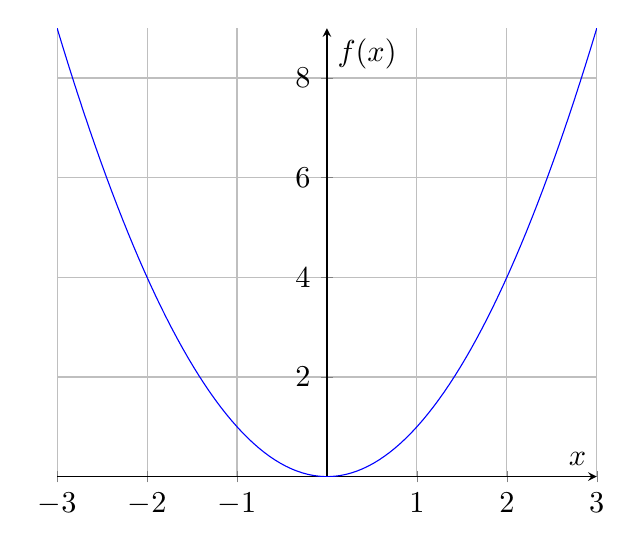
\begin{tikzpicture}
    \begin{axis}[
        grid,
        axis lines = center,
        xlabel = \(x\),
        ylabel = {\(f(x)\)},
        ]
    \addplot [
    domain=-3:3,
    samples=100,
    color=blue,
    ]
    {x^2};
    \end{axis}
\end{tikzpicture}

If you wanted, you could trace your finger along the graph of f(x) from $x=-3$ to $x=3$ without ever picking up your finger. This means the function is continuous in the domain from $-3 \leq x \leq 3$. In this case, the domain of continuity \textit{includes} the end points ($x=3$ and $x=-3$). This is called a closed interval. In other cases, the function will be continuous right up to, but not including, the endpoints, as with the domains of continuity for our other example, $g(x) = tanx$. This is called an open interval. Let's learn more about intervals of continuity by examining $g(x) = tanx$.

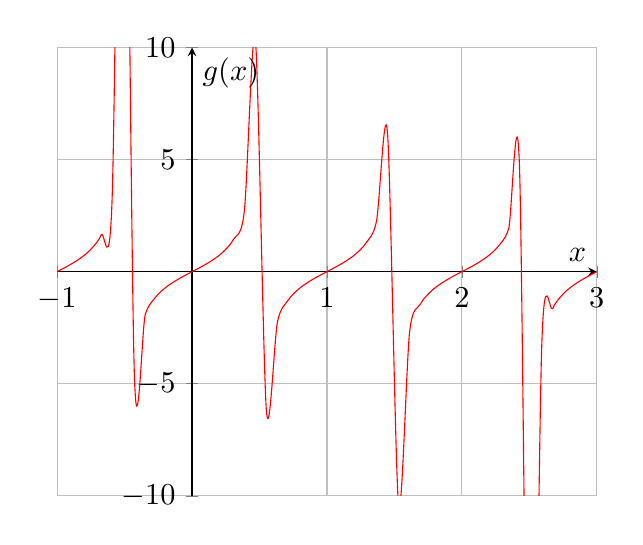
\begin{tikzpicture} %%FIXME make this graph prettier
    \begin{axis}[
        grid,
        axis lines = center,
        xlabel = \(x\),
        ylabel = {\(g(x)\)},
        ymin=-10,
        ymax=10
        ]
    \addplot[
    domain=-1:3,
    samples=50,
    smooth,
    red] 
    {tan(deg(pi*x))};
    \end{axis}
\end{tikzpicture}

As you can see, if you trace your finger along the graph of the function starting at $x=0$, you can continue without lifting your finger to $x=\frac{\pi}{2}$. As you approach $x=\frac{\pi}{2}$ from the left, the value of $g(x)$ approaches $\infty$. In order to continue tracing the function PAST $x=\frac{\pi}{2}$, you have to lift your finger and bring it down to $-\infty$. The function then continues continuously again until $x=\frac{3\pi}{2}$. 

In the case of $g(x) = tan(x)$, the function is continuous on \textit{open intervals}, including the open interval $\frac{\pi}{2} < x < \frac{3\pi}{2}$.

There is a shorter way to represent open and closed domain intervals. We can represent that $f(x) = x^2$ is continuous on the closed interval $-3 \leq x \leq 3$ in the following way: $$x \in \left[3, -3 \right]$$

Which reads as ``x contained in the domain -3 to 3, inclusive''. That is, all the values from -3 to 3, including the endpoints. The inclusion of the endpoints is implied by the use of \textit{brackets}. For open intervals, we use parentheses to communicate that the interval goes up to, but does not include, the endpoints. 

Formally, a function $f(x)$ is continuous at $x=a$ if $\lim_{x\to a}f(x)$ exists \textit{and} $\lim_{x\to a}f(x) = f(a)$. That is, the limit is equal to the actual value of the function. Re-examine the graph of $h(x)$. We have already seen that $\lim_{x\to 0}h(x)$ exists and is equal to 3. However, $h(0) = 2 \neq \lim_{x\to0}h(x)$. So h(x) is not continuous at x = 0. Because $-x^2+3$ is evaluable all the way to $-\infty$ and $-x+3$ is evaluable all the way to $\infty$, the fucntion h(x) is continuous everywhere \textit{except} $x=0$. We can represent this mathematically by saying $h(x)$ is continuous on the domain $x \in \left(-\infty, 0\right)\cup \left(0, \infty\right)$. We use parentheses for $\pm\infty$ because we can never actually reach $\infty$. Additionally, the function is continuous up to, but not including $0$, and the use of parentheses excludes $x=0$ from the domain of continuity.

There are some mathematical properties of limits which allow us to determine the limit of complex functions without seeing a graph or using a calculator to generate a table. 

The following laws are true given that \textit{c} is a constant, $\lim_{x\to\infty} f(x) $ exists, and $\lim_{x\to\infty} g(x) $ exists.

\begin{enumerate}
    \item Sum Law $\lim_{x\to\infty} \left[f(x) + g(x) \right] = lim_{x\to\infty} f(x) + lim_{x\to\infty} g(x)$
    \item Difference Law $\lim_{x\to\infty} \left[f(x) - g(x) \right] = lim_{x\to\infty} f(x) - lim_{x\to\infty} g(x)$
    \item Constant Multiple Law $lim_{x\to\infty} \left[\textit{c}f(x) \right] = \textit{c} \cdot lim_{x\to\infty}    f(x) $
    \item Product Law $lim_{x\to\infty} \left[f(x)g(x) \right] = lim_{x\to\infty}f(x) \cdot lim_{x\to\infty} g(x)$
    \item Quotient Law $lim_{x\to\infty} \frac{f(x)}{g(x)} = \frac{lim_{x\to\infty} f(x)}{lim_{x\to\infty} g(x)}$ given that $lim_{x\to\infty} g(x) \neq 0$
\end{enumerate}

These laws are fairly obvious - the limit of the sum of two functions is equal to the sum of the limits of each function individually. The only tricky on is the last: the limit of the quotient of two functions is equal to the quotient of the limits if and only if the limit of the function in the denominator does not equal zero. This makes sense, since we know dividing by zero yields an undefined result. 

Let's practice applying these laws to evaluate the limits of the functions f(x), shown in blue below, and g(x), shown in red below:

$f(x) = \begin{cases}
    -x^2+3, \text{ if } x \leq 0\\
    -x, \text{ if } x > 0
\end{cases}$

$g(x) = \begin{cases}
   x^2+1, \text{ if } x < 1 \\
    (x-2)^2, \text{ if } x \geq 1
\end{cases}$

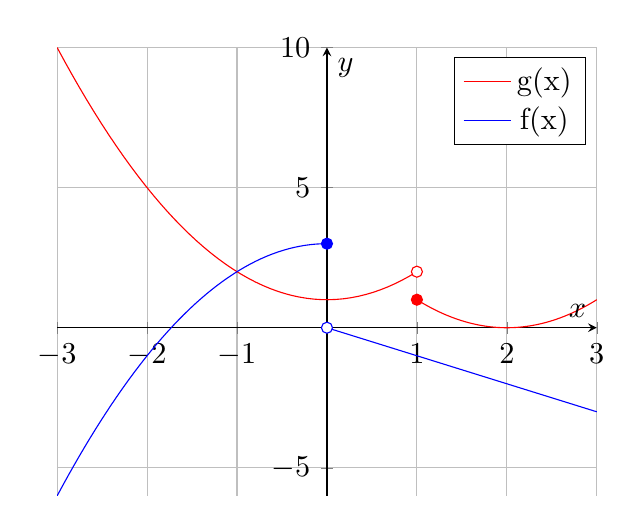
\begin{tikzpicture}
    \begin{axis}[
        grid,
        axis lines = center,
        xlabel = \(x\),
        ylabel = {\(y\)},
        ]
    \addplot [
    domain=-3:1,
    samples=50,
    color=red,
    ]
    {x^2+1};
    \addlegendentry{g(x)};
    \addplot[
    domain=-3:0,
    samples=50,
    color=blue,
    ]
    {-x^2+3};
    \addlegendentry{f(x)};
    \addplot[
    domain=1:3,
    samples=50,
    color=red,
    ]
    {(x-2)^2};
    \addplot[mark=*,fill=red,draw=red] coordinates{(1,1)};
    \addplot[mark=*,fill=white,draw=red] coordinates{(1,2)};
    
    \addplot[mark=*,fill=blue,draw=blue] coordinates{(0,3)};
    \addplot[mark=*, fill=white,draw=blue] coordinates{(0,0)};
    \addplot[
    domain=0:3,
    samples=50,
    color=blue,
    ]
    {-x};
    \end{axis}
\end{tikzpicture}

Limit Laws Practice, Part I:
Use the graphs of f(x) and g(x) given above to evaluate each limit, if it exists. If the limit does not exist, explain why. Two examples are given first:

Example 1: evaluate $\lim_{x\to0} f(x) \cdot g(x)$
From the Product Law, we know that:
$$\lim_{x\to0} f(x) \cdot g(x) = \lim_{x\to0}f(x) \cdot \lim_{x\to0} g(x)$$
Looking at the graph, we can see that $$\lim_{x\to0}g(x) = 1$$ and there is a discontinuity in $f(x)$ at $x=0$. Therefore, $$\lim_{x\to0}f(x) = \text{undef}$$ Substituting this, we get: $$\lim_{x\to0}f(x) \cdot \lim_{x\to0} g(x) = \text{undef} \cdot 1 = \text{undef}$$ Therefore, \textbf{the limit does not exist}. 

Example 2: evaluate $\lim_{x\to2}f(x) - g(x)$

Applying the Difference Law, we see that:

$$\lim_{x\to2}f(x) - g(x) = \lim_{x\to2}f(x) - \lim_{x\to2}g(x)$$

Examining the graph, we see that $$\lim_{x\to2}f(x) = -2$$ and $$\lim_{x\to2}g(x) = 0$$ Substituting these values, we get:

$$\lim_{x\to2}f(x) - g(x) = -2 - 0 = -2$$

Practice problems:
\begin{enumerate}
    \item $\lim_{x\to-3} \frac{f(x)}{g(x)}$
    \item $\lim_{x\to2}\left[f(x) + 5g(x)\right]$
    \item $\lim_{x\to-1} \frac{3g(x)}{f(x)}$
    \item $\lim_{x\to0}f(x) \cdot 5g(x)$
    \item $\lim_{x\to-1} f(x) - 3g(x) $
\end{enumerate}

Recall that exponents represent repeated multiplication. Therefore, if we apply the Product Law multiple times, we obtain the Power Law for limits:
\begin{enumerate}
    \setcounter{enumi}{5}
    \item Power Law $\lim_{x\to\infty} \left[f(x)\right]^n = \left[\lim_{x\to\infty}f(x)\right]^n$ where n is a positive integer
\end{enumerate}
There are two special limits that will be useful to us which are intuitively obvious, but we won't formally prove here.  
\begin{enumerate}
    \setcounter{enumi}{6}
    \item $\lim_{x\to a} \textit{c} = \textit{c}$
    \item $\lim_{x\to a} x = a$
\end{enumerate}
Combining Law 8 with the Power Law, we find that:
\begin{enumerate}
\setcounter{enumi}{8}
    \item $\lim_{x\to a} x^n = a^n$
\end{enumerate}
And similarly, for square roots:
\begin{enumerate}
    \setcounter{enumi}{9}
    \item $\lim_{x\to a} \sqrt[n]{x} = \sqrt[n]{a}$ (if n is even, we assume $a > 0$)
\end{enumerate}

Solutions to practice problems:

1. From the quotient law, we know that:$$\lim_{x\to3}\frac{f(x)}{g(x)}=\frac{\lim_{x\to3}f(x)}{\lim_{x\to3}g(x)}$$
From the graph, we see that: $$\lim_{x\to3}f(x) = -3$$
and that:$$\lim_{x\to3}g(x) = 1$$
Substituting these values, we get:
$$\lim_{x\to3}\frac{f(x)}{g(x)}=\frac{-3}{1} = -3$$


2. From the Sum Law, we know that: $$\lim_{x\to2}\left[f(x) + 5g(x)\right]=\lim_{x\to2}f(x) + \lim_{x\to2}5g(x)$$
and applying the Constant Multiple Law, we see that:
$$\lim_{x\to2}\left[f(x) + 5g(x)\right]=\lim_{x\to2}f(x) + 5\lim_{x\to2}g(x)$$
Examining the graph of f(x) and g(x), we can determine that $$\lim_{x\to2}f(x) = -2$$
and
$$\lim_{x/to2}g(x) = 0$$
Substituting these values, we get:
$$\lim_{x\to2}\left[f(x) + 5g(x)\right]=-2 + 5 \cdot 0 = -2$$


3.From the quotient law, we see that: $$\lim_{x\to-1} \frac{3g(x)}{f(x)}=\frac{\lim_{x\to-1}3g(x)}{\lim_{x\to-1}f(x)}$$

Applying the Constant Multiple Law, we get:
$$\lim_{x\to-1} \left[\frac{3g(x)}{f(x)}\right]=\frac{3\lim_{x\to-1}g(x)}{\lim_{x\to-1}f(x)}$$
From the graph, we see that:
$$\lim_{x\to-1}f(x) = 2$$
and
$$\lim_{x\to-1}g(x) = 2$$
Substituting, we get:
$$\lim_{x\to-1} \left[\frac{3g(x)}{f(x)}\right]=\frac{3 \cdot 2}{2}=3$$

4. Applying the Product and Constant Multiple Laws, we get:
$$\lim_{x\to0}\left[f(x) \cdot 5g(x)\right] = \lim_{x\to0}f(x) \cdot 5 \cdot \lim_{x\to0}g(x)$$
Examining the graphs, we see that $\lim_{x\to0}f(x)$ does not exist and $\lim_{x\to0}g(x) = 1$. Because $\lim_{x\to0}f(x)$ does not exist, $\lim_{x\to0}f(x) \cdot 5 \cdot \lim_{x\to0}g(x)$ also does not exist. 

5. Applying the Difference and Constant Multiple Laws, we see that:
$$\lim_{x\to-1} \left[f(x) - 3g(x)\right] =\lim_{x\to-1}f(x) - 3 \cdot \lim_{x\to-1}g(x)$$
Examining the graphs, we see that:
$$\lim_{x\to-1}f(x) = 2$$
and
$$\lim_{x\to-1}g(x) = 2$$
Substituting, we get that:
$$\lim_{x\to-1} \left[f(x) - 3g(x)\right] =2 - 3 \cdot 2 = 2-6 = -4$$

%Here is a function:
%
%$$f(x) = \frac{x^2}{x} + 1$$
%
%This $f$ is defined for any real number \emph{except 0}. (You can't
%divide anything, including zero, by zero.)
%
%Let's plot $f$:
%
%\begin{tikzpicture}[
%tl/.style = {% tick labels
%    fill=white, inner sep=1pt, font=\scriptsize,
%            },                        ]
%% grid
%\draw[sdkblue, very thin] (-3,-3) grid (3,3);
%
%
%    \draw[<->,thick,dashed] (-3.2,0) -- (3.2,0) node[right] {$x$};
%    \draw[<->,thick,dashed] (0,-3.2) -- (0, 3.2) node[above] {$y$};
%% curve
%\draw[<-,draw=black,thick,domain=-3:-0.1,samples=300,variable=\x] plot (\x,{\x + 1});
%\draw[thick] (0,1) circle (0.1);
%\draw[->,draw=black,thick,domain=0.1:2,samples=300,variable=\x] plot (\x,{\x + 1});
%\end{tikzpicture}
%
%You can see that the function is the same as $x + 1$ everywhere except
%$x = 0$.  You can see that as the function approaches $x=0$ from the
%left, the value of the function approaches 1.  You can see that as the
%function approaches $x=1$ from the right, the value of the function
%approaches 1.
%
%Mathematicians say ``The \newterm{limit} of $f$ as $x$ approaches 0, is 1.''  We have a notation for this:
%
%$$\lim_{x \rightarrow 0} f(x) = 1$$
%
%We generally use limit whenever we mean ``We are getting arbitrarily
%close, but we can never really get there.''  For example, you might
%say ``The limit of $1/t$ as $t$ goes to infinity is 0.''
%
%\begin{tikzpicture}[
%tl/.style = {% tick labels
%    fill=white, inner sep=1pt, font=\scriptsize,
%            },                        ]
%% grid
%\draw[sdkblue, very thin] (-5,-5) grid (5,5);
%    \draw[<->,thick,dashed] (-5.2,0) -- (5.2,0) node[below] {$t$};
%    \draw[<->,thick,dashed] (0,-5.2) -- (0, 5.2);
%% curve
%\draw[<->,draw=black,thick,domain=0.2:5,samples=300,variable=\x] plot (\x,{1/\x});
%\draw[<->,draw=black,thick,domain=-5:-0.2,samples=300,variable=\x] plot (\x,{1/\x});
%\draw (5.0, 0.2) node[above] {$t \rightarrow \infty$, $1/t \rightarrow 0$};
%\draw (0.0, 5.2) node[above] {$t \rightarrow 0$ from the right, $1/t \rightarrow \infty$};
%\draw (0.0, -5.2) node[below] {$t \rightarrow 0$ from the left, $1/t \rightarrow -\infty$};
%\draw (-5.0, -0.2) node[below] {$t \rightarrow -\infty$, $1/t \rightarrow 0$};
%
%\end{tikzpicture}
%
%What is the limit of $1/t$ as $t$ approaches zero? The limit isn't
%defined because if you approach from the right, $1/t$ goes to
%infinity, but if you approach from the left, $1/t$ goes to negative
%infinity.

\graphicspath{{../../Chapters/rational_functions/en_US}}
\chapter{Rational Functions}

We have discussed addition, subtraction, and multiplication of polynomials. What about division?

A quotient of polynomials is called a rational expression.\index{rational!expression} When the polynomials are factored and the stars align, we can simplify the rational expression to a single polynomial, just like we might reduce a fraction to lowest terms.

\textbf{Example} 
\begin{equation} \label{eq1}
\begin{split}
\frac{(x + 1)(x + 5)}{x + 5} & = (x + 1) \cdot \frac{x+5}{x+5} \\
& = x + 1 \qquad (x\ne5)
\end{split}
\end{equation}\footnote{It is important to note that we need to restrict $x=5$ since this would be division by zero. FIXME expand on this?}

What if the polynomials are not factored? Factor them first.

\textbf{Example} 
\[ \frac{x^2 + 6x + 5}{x + 5} = \frac{(x + 1)(x + 5)}{x + 5} \]
and simplify as in the previous example.

Now, let us consider a rational expression which can be simplified to a single polynomial --- but in the denominator.

\textbf{Example}
\begin{equation} \label{eq1}
\begin{split}
\frac{x + 5}{x^2 + 6x + 5} & = \frac{x + 5}{(x + 1)(x + 5)} \\
& = \frac{1}{x+1} \cdot \frac{x+5}{x+5} \\
& = \frac{1}{x+1} \\
\end{split}
\end{equation}

Consider this expression as a function: \( f(x) = \frac{1}{x+1} \). As you might have guessed, this is called a rational function.\index{rational!function} We did not bother looking at the result of the previous example as a function, because we already know that function type: it is a line with slope \( 1 \) and y-intercept \( 1 \). However, this rational function is another animal entirely. Let us examine our first rational function with a familiar concept: the y-intercept. 

y-intercept: \( f(0) = \frac{1}{0 + 1} = \frac{1}{1} = 1 \). The graph contains the point \( (0, 1) \).

Does \( f \) have an x-intercept? That would be an \( x \)-value where \( f(x) = 0 \). But a fraction equals \( 0 \) only when its numerator equals \( 0 \); since the numerator of this expression is always \( 1 \), \( f \) has no x-intercept. 

Knowing the \( y \)-intercept, and that there is no \( x \)-intercept, is a comforting start. But things get weird when we consider a concept that has previously seemed quite simple: domain. Recall that the domain of a function is the set of all values which can be used as inputs. In this case, the domain includes all real numbers, with one exception. The number \( -1 \) is not a valid input because \( f(-1) = \frac{1}{-1+1} = \frac{1}{0} \), which is undefined. So, we say that the domain is all real numbers except \( -1 \). This means the graph contains a point corresponding to every \( x \)-value except \( -1 \).

There is no point at \( x = -1 \), but there is a point at every other \( x \)-value, such as, for example, \( -1.1 \), or \( -0.99999 \). So, what is happening near \( x = -1 \)?

\begin{center}
\begin{tabular}{ |c|c|c|c|c|c|c| } 
 \hline
 x & -1.1 & -1.01 & -1.001 & -0.999 & -0.99 & -0.9 \\ 
 \hline
 f(x) & -10 & -100 & -1000 & 1000 & 100 & 10 \\ 
 \hline
\end{tabular}
\end{center}

The function is going haywire. As we choose \( x \)-values closer and closer to \( -1 \), the resulting function values are larger and larger in magnitude. Also, they are negative on one side, but positive on the other. So, how does a graph go from \( y \)-values of \( -10 \), to \( -100 \), to \( -1000 \), all in a space of less than \( 0.1 \) on the \( x \)-axis? Then, from there, suddenly to big positive numbers on the other side of \( x = -1 \)? All without ever crossing the \( x \)-axis (since there is no \( x \)-intercept)? Let's look at the graph.

\begin{figure}[htbp]
  \centering
  \begin{tikzpicture}
    \begin{axis}[
      axis lines = middle,
      xlabel = \(x\),
      ylabel = \(f(x)\),
      restrict y to domain = -10:10,
      samples = 100,
    ]
    \addplot [blue, smooth] {1/(x + 1)};
    \end{axis}
  \end{tikzpicture}
  \caption{Graph of \( f(x) = \frac{1}{x+1} \)}
\end{figure}

We can see the \( y \)-intercept we found above. We can also see that the graph has no \( x \)-intercept, as expected. The phenomenon occurring at \( x = -1 \) is called a vertical asymptote.\index{vertical!asymptote} One other interesting feature of this graph is how it hugs the \( x \)-axis toward the left and right edges of the window. This makes the line \( y = 0 \) (the \( x \)-axis) a horizontal asymptote for this function.\index{horizontal!asymptote} We can see why this is happening numerically by considering what happens for \( x \)-values far from \( 0 \). In this function, the result is a fraction with a numerator of \( 1 \) and a denominator that is large in size: a fraction that is close to \( 0 \).

\begin{center}
\begin{tabular}{ |c|c|c|c|c|c|c| } 
 \hline
 x & -1000 & -100 & -10 & 10 & 100 & 1000 \\ 
 \hline
 f(x) & -0.001 & -0.01 & -0.1 & 0.1 & 0.01 & 0.001 \\ 
 \hline
\end{tabular}
\end{center}

Let's examine another rational function. Begin by factoring to see if the function can be simplified.
\[ g(x) = \frac{x^2 - 3x + 2}{x^2 - 4x + 3} = \frac{(x - 1)(x - 2)}{(x - 1)(x - 3)} \]
Consider the domain of \( g \) before continuing. Which values of \( x \) are valid inputs? Since substituting \( x = 1 \) or \( x = 3 \) would result in division by \( 0 \), these are not valid inputs. The domain of \( g \) is all real numbers except \( 1 \) and \( 3 \).

Now, for any \( x \)-value except \( 1 \), \( \frac{x-1}{x-1} = 1 \). This means that, for all \( x \)-values but \(1\), we can cancel those factors, leaving \( g(x) = \frac{x-2}{x-3} \). (We will talk more about what is happening at \( x = 1 \) in a moment.)

This function has both \( x \)- and \( y \)-intercepts:
\( y \)-intercept: \( g(0) = \frac{0-2}{0-3} = \frac{2}{3} \). The graph contains the point \( (0, \frac{2}{3}) \).
\( x \)-intercept: \( g(x) = 0 \) where the numerator equals \( 0 \) and the denominator does not equal \( 0 \). Since \( x - 2 = 0 \) when \( x = 2 \), the \( x \)-intercept is \( 2 \) and the graph contains the point \( (2, 0) \).

The graph of \( g \) has a vertical asymptote at any \( x \)-value where substitution would result in dividing a nonzero number by zero. Thus, \( g \) has a vertical asymptote at \( x = 3 \).

Does \( g \) have a horizontal asymptote? Let us see what happens when we substitute \( x \)-values far from \( 0 \).

\begin{center}
\begin{tabular}{ |c|c|c|c|c|c|c| } 
 \hline
 x & -1000 & -100 & -10 & 10 & 100 & 1000 \\ 
 \hline
 g(x) & 0.999 & 0.990 & 0.923 & 1.143 & 1.010 & 1.001 \\ 
 \hline
\end{tabular}
\end{center}

As we move further away from the \( y \)-axis, the \( y \)-values become closer to \( 1 \). The horizontal asymptote describes the end behavior of the function, or what the graph looks like far from the \( y \)-axis.\index{end!behavior} In this case, if we ignore the portion close to the \( y \)-axis, the graph begins to look like the line \( y = 1 \), making this the horizontal asymptote of \( g \). 

So, what is happening at \( x = 1 \)? The value is not in the domain of the function, but there is no vertical asymptote there. That is because substituting any other value for \( x \), even values very close to \( 1 \), into \( \frac{(x - 1)(x - 2)}{(x - 1)(x - 3)} \) gives the exact same number as substituting into \( \frac{x-2}{x-3} \). So, there is a hole in the graph at \( x = 1 \), but nothing strange is happening on either side of \( 1 \).\index{hole} (Depending on the graphing software, the hole may not be visible.)

\begin{figure}[htbp]
  \centering
  \begin{tikzpicture}
    \begin{axis}[
      axis lines = middle,
      xlabel = \(x\),
      ylabel = \(g(x)\),
      restrict y to domain = -10:10,
      samples = 100,
    ]
    \addplot [red, smooth] {(x - 2)/(x - 3)};
    \end{axis}
  \end{tikzpicture}
  \caption{Graph of \( g(x) = \frac{x^2 - 3x + 2}{x^2 - 4x + 3} \)}
\end{figure}

\begin{Exercise}[title=Rational Functions Practice 1, label=ratfunc1]
  Determine the x- and y-intercepts and horizontal and vertical asymptotes of the rational function:
  \Question{$\frac{2x + 5}{x + 4}$}
  \vspace{40mm}
\end{Exercise}
\begin{Answer}[ref=ratfunc1]
x-intercept: $(-5/2, 0)$; y-intercept: $(0, 5/4)$; horizontal asymptote: $y = 2$; vertical asymptote: $x = -4$
\end{Answer}

\begin{Exercise}[label=ratfunc2]
	[This question was originally presented in the no-calculator section 
	of the 2012 AP Calculus BC exam.] The line $y = 5$ is a horizontal 
	asymptote of which of the following functions? Explain. \\
	A. $y = \frac{\sin{5x}}{x}$\\
	B. $y = 5x$\\
	C. $y = \frac{1}{x-5}$\\
	D. $y = \frac{5x}{1-x}$\\
	E. $y = \frac{20x^2 - x}{1 + 4x^2}$
\end{Exercise}

\begin{Answer}[ref=ratfunc2]
	The correct answer is E. To explain, we examine the behavior of each 
	function as $x \to \infty$. \\
	A. $\lim_{x \to \infty} \frac{\sin{5x}}{x} = \pm \infty \neq 5$\\
	B. $\lim_{x \to \infty} 5x = \infty \neq 5$\\
	C. $\lim_{x \to \infty} \frac{1}{x-5} = 0 \neq 5$ (this function 
	does have a \textit{vertical} asymptote at $x = 5$). \\
	D. $\lim_{x \to \infty} \frac{5x}{1-x} = \frac{5}{-1} = -5 \neq 5$ 
	(this function has a horizontal asymptote at $x = -5$).\\
	E. $\lim_{x \to \infty} \frac{20x^2 - x}{1 + 4x^2} = \frac{20}{4} = 5$. 
\end{Answer}

In those examples, common factors cancel, leaving one polynomial. Of course, there is no guarantee that any two polynomials will have common factors, or even be factorable at all. Now, we consider an example that cannot be simplified. We will focus on just the asymptotes here.
\[ h(x) = \frac{x^2}{x - 1} \]
We see that the \( x \)-value \( 1 \) gives division of a non-zero number by zero, giving a vertical asymptote at \( x = 1 \). How about a horizontal asymptote? We examine values of \( h \) for values of \( x \) far from \( 0 \).

\begin{center}
\begin{tabular}{ |c|c|c|c|c|c|c| } 
 \hline
 x & -1000 & -100 & -10 & 10 & 100 & 1000 \\ 
 \hline
 h(x) & -999 & -99 & -9 & 11 & 101 & 1001 \\ 
 \hline
\end{tabular}
\end{center}

Rather than seeing function values leveling off as in the previous examples, we see function values that grow in size along with \( x \). The function \( h \) has no horizontal asymptote. Let's examine the graph:

\begin{figure}[htbp]
  \centering
  \begin{tikzpicture}
    \begin{axis}[
      axis lines = middle,
      xlabel = \(x\),
      ylabel = \(h(x)\),
      restrict y to domain = -10:10,
      samples = 100,
    ]
    \addplot [green, smooth] {x^2/(x - 1)};
    \end{axis}
  \end{tikzpicture}
  \caption{Graph of \( h(x) = \frac{x^2}{x - 1} \)}
\end{figure}

This function exhibits a different type of end behavior: that of a line with slope \( 1 \). To see that, cover up the portion of the graph near the \( y \)-axis and focus on the left and right. The rather dull and time-consuming technique of polynomial long division can be used to rewrite the function as a quotient and a remainder. We encourage you to watch the Khan Academy video on the topic, but for now, let us instead use our knowledge of factoring techniques and a clever little trick.

\begin{equation} \label{eq1}
\begin{split}
h(x) & = \frac{x^2}{x - 1} \\
& = \frac{x^2 - 1 + 1}{x - 1} \\ 
& = \frac{x^2 - 1}{x - 1} + \frac{1}{x - 1} \\
& = \frac{(x - 1)(x + 1)}{x - 1} + \frac{1}{x - 1} \\
& = x + 1 + \frac{1}{x - 1}
\end{split}
\end{equation}

We obtain a quotient of \( x + 1 \) and a remainder of \( 1 \). It is the quotient that determines the end behavior of the graph. Why? Substituting \( x \)-values far from zero makes the remainder term very small, since it becomes a fraction with a large denominator but a numerator of only \( 1 \). So for \( x \)-values far from zero, the \( y \)-value is \( x \) plus \( 1 \) plus a very small number (so small that we can justifiably ignore it). This means that far from the \( y \)-axis, the function acts like the quotient: the line \( y = x + 1 \). We call this line an oblique asymptote.\index{oblique!asymptote} See below how the graph of \( h(x) \) hugs that line.

\begin{figure}[htbp]
  \centering
  \begin{tikzpicture}
    \begin{axis}[
      axis lines = middle,
      xlabel = \(x\),
      ylabel = \(y\),
      restrict y to domain = -10:10,
      samples = 100,
    ]
    \addplot [green, smooth] {x^2/(x - 1)};
    \addplot [black, dashed] {x + 1};    
    \end{axis}
  \end{tikzpicture}
  \caption{Graph of \( h(x) = \frac{x^2}{x - 1} \) and its oblique asymptote \( y = x + 1 \)}
\end{figure}

\begin{Exercise}[title=Rational Functions Practice 2, label=ratfunc2]
  Factor and simplify the rational function, then determine any holes and vertical and oblique asymptotes of the rational function.
  \Question{$\frac{x^3 + 2x^2}{x^2 + x}$}
  \vspace{40mm}
\end{Exercise}
\begin{Answer}[ref=ratfunc2]Factored form: $\frac{x^2(x + 2)}{x(x + 1)}$; hole: $(0, 0)$; vertical asymptote: $x = -1$; oblique asymptote: $y = x + 1$\end{Answer}

We have seen lines act as end behaviors. Are there other possibilities? Sure! Here is an example with parabolic end behavior. 
\[ k(x) = \frac{x^3}{x - 2} \]
We use our add-subtract trick to reveal the quotient, which describes the end behavior.

\begin{equation} \label{eq1}
\begin{split}
h(x) & = \frac{x^3}{x - 2} \\
& = \frac{x^3 - 8 + 8}{x - 2} \\ 
& = \frac{x^3 - 8}{x - 2} + \frac{8}{x - 2} \\
& = \frac{(x - 2)(x^2 + 2x + 4)}{x - 2} + \frac{8}{x - 2} \\
& = x^2 + 2x + 4 + \frac{8}{x - 2}
\end{split}
\end{equation}

The quotient, \( x^2 + 2x + 4 \), should describe the end behavior. We confirm by graphing both \( k \) and the quotient - the parabolic asymptote.

\begin{figure}[htbp]
  \centering
  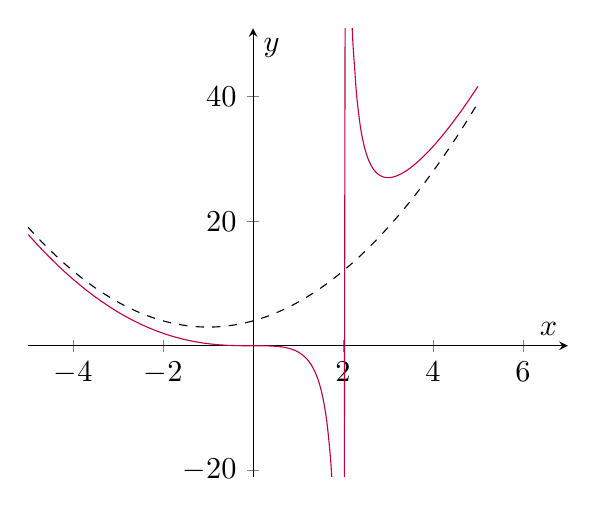
\begin{tikzpicture}
    \begin{axis}[
      axis lines = middle,
      xlabel = \(x\),
      ylabel = \(y\),
%      restrict y to domain = -10:10,
      samples = 100,
      xmin = -5, xmax = 7, ymin = -21, ymax = 51,
    ]
    \addplot [purple, smooth] {x^3/(x - 2)};
    \addplot [black, dashed] {x^2 + 2*x + 4};    
    \end{axis}
  \end{tikzpicture}
  \caption{Graph of \( k(x) = \frac{x^3}{x - 2} \) and its parabolic asymptote \( y = x^2 + 2x + 4 \)}
\end{figure}
%%%%%%%%%%%%%%%%%%%%%%%%%%%%%%%%%
%% Bookfooter.tex by Aaron Hillegass
%% Nov 8, 2020

\appendix

\chapter{Answers to Exercises}
\shipoutAnswer

\bibliography{references}

\printindex

\end{document}